\section{Application: Community detection}
\label{sec:communities}

In many cases, such as online networks, 
we would like to be able to recover specific communities in those graphs.
In the typical setup, a community is a set of vertices that are more densely connected
together than to the rest of the graph.

The model we present here
is inspired by the planted partition or
stochastic blockmodel (SBM, \citet*{holland1983}).
In the SBM, each vertex belongs to a class or community, 
and the probability that two vertices are connected is a function
of the classes of the  vertices.
It is a generalization of the \ER random graph.
The classes or blocks in the SBM make it a good model for
graphs with community structure, 
where nodes preferentially connect to other nodes
depending on their communities
(\citet*{newman2010}).

There are many methods for detecting a community given a graph.
For an overview of the topic, see \citet*{fortunato2010}.
Spectral clustering is a common method which can be applied to any set of data
$\{ \zeta_i \}_{i=1}^n$.
Given a symmetric and non-negative similarity function $S$,
the similarity is computed for every pair of data points, forming a matrix
$A_{ij} = S(\zeta_i, \zeta_j ) = S(\zeta_j, \zeta_i ) \geq 0$.
The spectral clustering technique is to compute the leading eigenvectors of
$A$, or matrices related to it, and use the eigenvectors to cluster the data.
In our case, the matrix in question is just the 
Markov matrix of a graph, defined soon.
We will show that we can guarantee the success of the technique if the degrees
are large enough.

Our graph model is a regular version of the SBM.
We build it on a ``frame,''
which is a small, weighted graph that
defines the community structure present in the larger, random graph.
Each class is represented by a vertex in the frame.
The edge weights in the frame define the number of edges
between classes.
What makes our model differ from the SBM is that
the connections between classes are described by a 
regular random graph rather than an \ER random graph.
However, the graph itself is not necessarily regular.

A number of authors have studied similar models.
Our model is a generalization of a random lift of the frame,
which is said to {\it cover} the random graph
(e.g. \citet*{marcus2013a,angel2015,bordenave2015a}).
This type of random graph was also studied by 
\citet*{newman2014}, who called it an equitable random graph,
since the community structure is equivalent to an 
equitable partition.
This partition induces a number of symmetries across vertices in 
each community which are useful when studying the 
eigenvalues of the graph.
\citet*{barrett2017} studied the effect of these symmetries 
from a group theory standpoint.
The work of \citet*{barucca2017} is closest to ours:
they consider spectral properties of such graphs and their 
implications for spectral community clustering. 
In particular, they show that the spectrum of what we call the ``frame'' 
(in their words, the discrete spectrum, which is deterministic) 
is contained in that of the random graph.
They use the resolvent method
(called the cavity method in the physics community)
to analyze the continuous part of the spectrum in the limit of
large graph size, and argue that community detection is possible
when the deterministic frame eigenvalues all lie outside the bulk.
However, this analysis assumes that there are no stochastic 
eigenvalues outside the bulk, which will only hold with high probability
if the graph is Ramanujan.
Our analysis shows that, if a set of pairwise spectral gaps hold between
all communities, then this will be the case.


\subsection{The frame model}

We define the {\it \kframe} distribution 
$\mathcal{G}(n,H)$
as a distribution of simple graphs on $n$ 
vertices parametrized by the ``frame'' $H$.
The frame $H=(V,E,p,D)$
is a weighted, directed graph.
Here, $V$ is the vertex set,
$E \subseteq \{(i,j): i,j \in V\}$ 
is the directed edge set,
the vertex weights are $p$, and the edge weights are $D$.
Note that we drop the arrows on the edge set in this Section, 
since it will always be directed.
The vertex weight vector
$p \in \R^{|V|}$, 
where
$\sum_{i \in V} p_i = 1$,
sets the relative sizes of the classes.
The edge weights are a matrix of degrees
$D \in \mathbb{N}^{|V| \times |V|}$.
These assign the number of edges between each class in the random graph:
$D_{ij}$
is the number of edges from each vertex in class $i$
to vertices in class $j$.
The degrees must satisfy the
balance condition
\begin{equation}
  \label{eq:detailedbalance}
  p_i D_{ij} = p_j D_{ji}
\end{equation}
for all
$i,j \in V$ where $(i,j)$ or $(j,i)$ are in $E$.
This requires that, for every edge $e \in E$,
its reverse orientation also exists in $H$.
We also require that
$n_i = n p_i \in \mathbb{N}$
for every $i \in V$, 
so that the number of vertices in each type is integer.

Given the frame $H$,
a \kframe $G \sim \mathcal{G}(n,H)$
is a simple graph on $n$ vertices with $n_i$
vertices in class $i$.
It is chosen uniformly among graphs 
with the constraint that each vertex in class $i$ makes
$D_{ij}$ connections among the vertices in class $j$.
In other words, if $i = j$, we sample that block of the adjacency
matrix as the adjacency matrix of a $D_{ii}$-regular random graph
on $n_i$ vertices.
For off-diagonal blocks $i \neq j$,
these are sampled as bipartite, biregular random graphs
$\mathcal{G} (n_i, n_j, D_{ij}, D_{ji})$.

\begin{figure}[t!]
  {\bf \Large A}\qquad {\large Frame}
  \hspace{2.05in}
  {\bf \Large B}\qquad {\large Random regular frame graph}
  \begin{center}
  \hspace{.34in}
  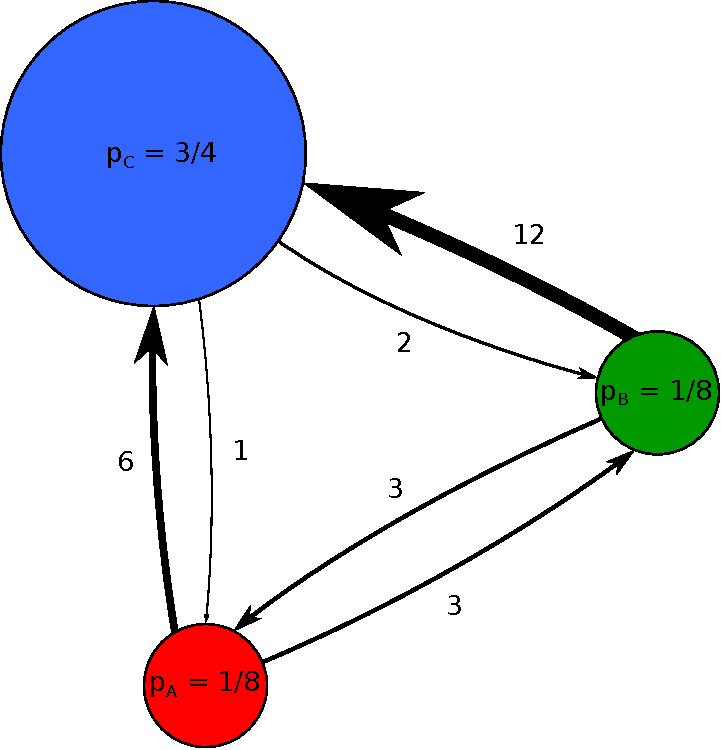
\includegraphics[height=2.6in]{frame.pdf}
  \hfill
  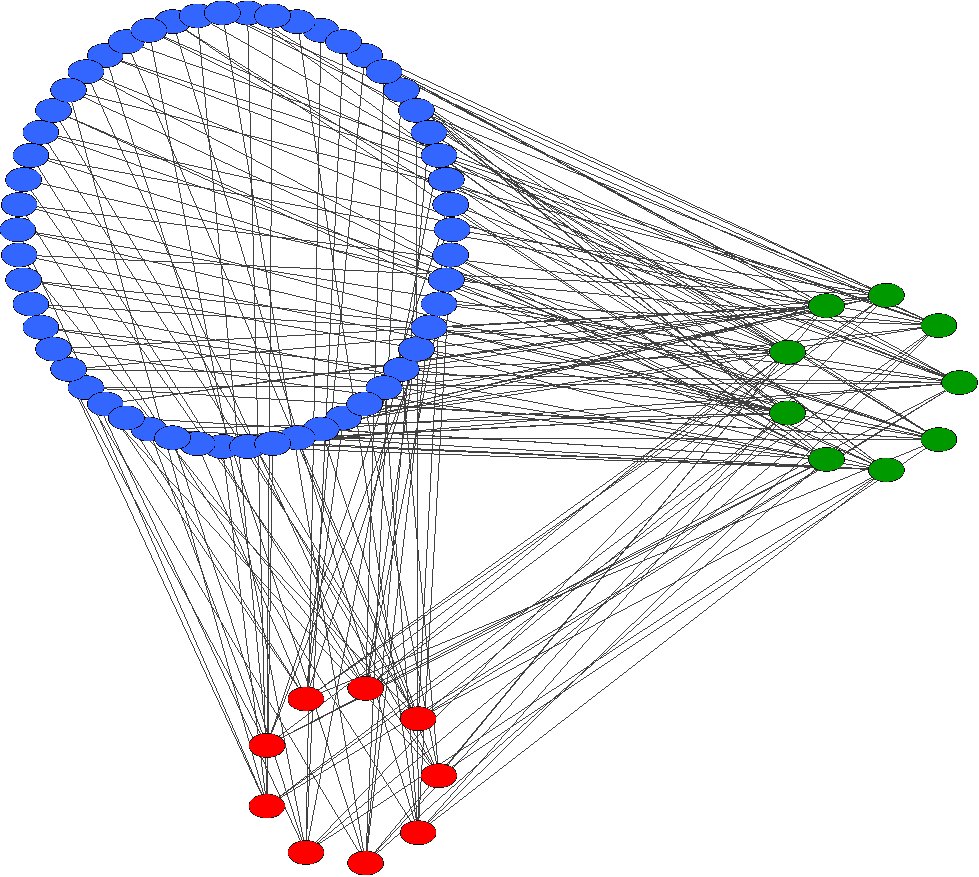
\includegraphics[height=2.6in]{small_tripartite.pdf}
\end{center}
  \caption{Schematic and realization of a \kframe. 
    {\bf A}, 
    the frame graph.
    The vertices of the frame (red = A, green = B, blue = C)
    are weighted according to their proportions $p$
    in the \kframe.
    The edge weights $D_{ij}$ 
    set the between-class vertex degrees
    in the \kframe.
    This frame will yield a random tripartite graph.
    {\bf B}, realization of the graph on 72 vertices. 
    In this instance, there are 
    $1/8 \times 72=9$ green and red vertices
    and
    $3/4 \times 72=54$ blue vertices.
    Each blue vertex connects to 
    $k_{CA}=1$ red vertex and
    $k_{CB}=2$ green vertices.
    This is actually a multigraph; 
    with so few vertices, the probability that
    the configuration model algorithm yields parallel edges is high.
  }
  \label{fig:frame}
\end{figure}

Sampling from 
$\mathcal{G}(n,H)$
can be performed similar to the configuration model,
where each node is assigned as many half-edges as its degree,
and these are wired together with a random matching 
(\citet*{newman2010}).
The detailed balance condition 
Eqn.~\eqref{eq:detailedbalance} 
ensures that this matching is possible.
Practically, we often have to generate many candidate matchings
before the resulting graph is simple, 
but the probability of a simple graph is bounded away from zero for
fixed $D$.

An example of a \kframe is the bipartite, biregular random graph.
The family $\mathcal{G}(n, m, d_1, d_2)$ 
is a \kframe $\mathcal{G}(n + m, H)$,
where the frame $H$ is the directed path on two vertices:
$V= \{ 1, 2 \}$ and $E = \{ (1,2), (2,1) \}$.
The weights are taken as 
$p_1 = n/(n+m)$, $p_2 = m/(n+m)$, $D_{12} = d_1$, and $D_{21} = d_2$.

Another example \kframe is shown in
Figure~\ref{fig:frame}.
In this case, the frame $H$ has 
$V= \{ A, B, C \}$ and 
$E = \{ (A,B), (A,C), (B,A), (B,C), (C,A), (C,B) \}$
with weights $p$ and $D$ as shown in Figure~\ref{fig:frame}A.
We see that this generates a random tripartite graph with 
regular degrees between vertices in different independent sets,
shown in Figure~\ref{fig:frame}B.

\subsection{Markov and related matrices of frame graphs}

Now, we define a number of matrices associated with the frame 
and the sample of the \kframe.

Let $G$ be a simple graph.
Define $D_G = \mathrm{diag}(d_G)$,
the diagonal matrix of degrees in $G$.
The Markov matrix $P=P(G)$ is defined as
\[
P = D_G^{-1} A,
\]
where $A=A(G)$ is the adjacency matrix.
The Markov matrix is the row-normalized adjacency matrix, and it contains
the transition probabilities of a random walker on the graph $G$.
Let $L = I - \mathcal{L} =  D_G^{-1/2} A \, D_G^{-1/2}$
be a matrix simply related to the normalized Laplacian.
We call this the {\it symmetrized Markov matrix}.
Then $P$ and $L$ have the same eigenvalues,
but $L$ is symmetric, since $L_{ij} = \frac{A_{ij}}{ \sqrt{ d_i d_j } }$. 

Suppose $G \sim \mathcal{G}(n, H)$, where the frame $H = (V,E,p, D)$.
Another matrix that will be useful is what we call the 
{\it Markov matrix of the frame}
$R$, where
$R_{ij} = \frac{ D_{ij} }{\sum_j D_{ij}}$.
% \[
% R = \mathrm{diag}(d)^{-1} D,
% \]
% where now $d_i = \sum_j d_{ij}$, 
Thus, $R$ is a row-normalized $D$, 
in the same way that the Markov matrix $P$ is the row-normalized adjacency matrix $A$.
Furthermore, $R$ is invariant under any uniform scaling of the degrees.
% $D \to \kappa D$.
Because of this equitable partition property of {\kframe}s, 
eigenvectors of the frame matrices $D=D(H)$ or $R=R(H)$ lift to 
eigenvectors of $A = A(G)$ or $P=P(G)$, respectively.
Suppose $D x = \lambda x$,
then it is a straightforward exercise to check that $A \tilde{x} = \lambda \tilde{x}$ 
for the piecewise constant vector
\[
\tilde{x} = 
\left[
\begin{array}{c}
\1_{n_1} x_1 \\
\1_{n_2} x_2 \\
\vdots
\end{array}
\right] .
\]
Using the same procedure, we can
lift any eigenpair of $R$ to an eigenpair of $P$ with the same eigenvalue.

\subsubsection{Bounds on the eigenvalues of frame graphs in terms of blocks}

The following result is due to \citet*{wan2015}:
\begin{proposition}
\label{thm:spurious_eig_bound}
Let $G$ be a random regular frame graph $G(n,H)$,
$P$ its Markov matrix, 
and $L$ the Laplacian
with vertices ordered by class in both cases.
% Define the vector $s \in \R^n$ by $s_i = \sqrt{d_i}$, 
% which is the Frobenius eigenvector of $L$ with eigenvalue 1.
Let $R$ be the Markov matrix of the frame $H=(V,E,p,D)$, 
with $|V(H)| = K$ classes.
% and $\lambda_1 \ge \ldots \ge \lambda_K$ the eigenvalues of $D$.
Define the matrices
$L^{(kl)}$
as the $(k,l)$ 
block of $L$ with respect to the clustering of vertices by class.
For $l \neq k$, let
\[
M^{(kl)} =
\left(
\begin{array}{cc} 
0 & L^{(kl)} \\
L^{(kl)} & 0 
\end{array}
\right) 
=
\left(
\begin{array}{cc} 
0 & L^{(kl)} \\
L^{(lk)*} & 0 
\end{array}
\right)
.
\]
For $l=k$, let $M^{(kk)} = L^{(kk)}$.
Assume that all eigenvalues of $D$ are nonzero and pick a constant $C$ such that
\[
	\frac{| \lambda_2^{(kl)} |}{\lambda_1^{(kl)}} \le C < 1
\]
for every $k,l = 1, \ldots K$, 
where $\lambda_1^{(kl)}$ and $\lambda_2^{(kl)}$ are the
leading and second eigenvalues of $M^{(kl)}$.
Under these conditions, the eigenvalues of $P$ which are not eigenvalues of $R$
%(spurious eigenvalues)
are bounded by 
\[
C \max_{k=1,\ldots, K} \left( R_{kk} + \sum_{l \neq k} \sqrt{R_{kl} R_{lk}} \right)
\leq \frac{C}{2}  \left(1 + \max_{k=1,\ldots, K} \sum_{l=1}^K R_{lk} \right) .
\]
\end{proposition}


The spectrum of the Markov matrix $\sigma(P)$ enjoys a simple connection to $\sigma(A)$ 
when $A$ is the adjacency matrix of a graph drawn from $G(n,m,d_1,d_2)$.
In this case, $L = \frac{ A }{ \sqrt{d_1 d_2} }$, 
so the eigenvalues of $P$ are just the scaled eigenvalues of $A$.
This and the spectral gap for bipartite, biregular random graphs, 
Theorem~\ref{cor:gap_A},
lead to the following remark:

\begin{remark}
For a random regular frame graph, 
$M^{(kl)}$ corresponds to the symmetrized Markov matrix $L$ 
of a bipartite biregular graph 
$G(n_k, n_l, D_{kl}, D_{lk})$.
Thus,
\[
\frac{| \lambda_2^{(kl)} |}{\lambda_1^{(kl)}} 
\leq
\frac{\sqrt{D_{kl} - 1} +\sqrt{D_{lk} - 1}}{\sqrt{D_{kl} D_{lk}}} + \epsilon .
\]
\end{remark}

Suppose we are given a frame that fits the conditions of 
Proposition~\ref{thm:spurious_eig_bound};
namely, $D$ cannot have any zero eigenvalues.
Then we can uniformly grow the degrees, which leaves $R$ invariant,
but allows us to reach an arbitrarily small $C$.
This ensures that the leading $K$ eigenvalues of $P$ are equal to the 
eigenvalues of $R$.
Note that this actually means that the entire \kframe satifsfies 
a weak Ramanujan property.
We now show that this guarantees spectral clustering.

\subsection{Spectral clustering}

Spectral clustering is a popular method of community detection.
Because some eigenvectors of $P$, the Markov matrix of a \kframe,
are piecewise constant on classes, 
we can use them to recover the communities so long as those eigenvectors can be identified.
Suppose there are $K$ total classes in our \kframe.
Then, given the eigenvectors $x^1, x^2, \ldots, x^K$, which are piecewise constant across classes,
we can cluster vertices by class.
For each vertex $v \in V(G)$, associate the vector
$y^v \in \R^K$
where $y^v_j = x^j_v$.
Then if $y^v = y^u$ for $u, v \in V(G)$, 
vertices $u$ and $v$ belong to the same class\footnote{
In the SBM case, the eigenvectors are not piecewise constant, 
but they are aligned with the eigenvectors of $R$
and thus highly correlated across vertices in the same class.
A more flexible clustering method such as $K$-means must be applied to the vectors $y$
in that case.
}.
It is simple to recover these piecewise constant vectors
$x^1, x^2, \ldots, x^K$ when they are the leading eigenvectors.
These facts lead to the following theorem:

\begin{theorem}[Spectral clustering guarantee in frame graphs]
\label{thm:spectral_clustering}
Let $G$ be a random regular frame graph $G(n,H)$
and $P$ its Markov matrix.
Let $R$ be the Markov matrix of the frame $H=(V,E,p,D)$, 
with $|V(H)| = K$ classes
and $\lambda_1 \ge \ldots \ge \lambda_K$ the eigenvalues of $R$
and $|\lambda_K| > 0$. 
Then we can scale the degrees by some $\kappa \in \mathbb{N}$,
$D \to \kappa D$,
so that the vertex classes are recoverable by spectral clustering of 
the leading $K$ eigenvectors of $P$.
\end{theorem}

\begin{remark}
The conditions of Theorem~\ref{thm:spectral_clustering},
while very general, are also weaker than may be expected using more sophisticated methods
tailored to the specific frame model. 
We illustrate this with the following example.
\end{remark}

\subsubsection{Example: The regular stochastic block model}

\citet*{brito2016} and \citet*{barucca2017} studied a regular stochastic block model,
which can be seen as a special case of our frame model.
Let the frame $H$ be the complete directed graph on two vertices, 
including self loops, where
\[
D = \left(
\begin{array}{cc}
d_1 & d_2\\
d_2 & d_1
\end{array}
\right)
\]
and $p = (1/2, 1/2)$.
Define the regular stochastic block model as $\mathcal{G} (2n, H)$.
This is a graph with two classes of equal size, 
representing two communities of vertices,
with within-class degree $d_1$ and between-class degree $d_2$. 
We assume $d_1 > d_2$, since communities are more strongly connected within.
\citet*{brito2016} proved the following theorem:
\begin{theorem}
\label{thm:RSBM_condition}
If $(d_1-d_2)^2 > 4 (d_1 + d_2 -1)$, then there is an efficient algorithm
for strong recovery, i.e.\ recovery of the exact communities with high probability
as $n \to \infty$.
\end{theorem}

Theorem~\ref{thm:RSBM_condition} gives a sharp bound on the degrees for recovery,
which we can compare to our spectral clustering results.
The eigenvalues of $D$ are $d_1 + d_2$ and $d_1 - d_2$,
and the Markov matrix of the frame $R$ has eigenvalues $1$ and $(d_1 - d_2) / (d_1 + d_2)$.
The diagonal blocks $L^{(11)}$ and $L^{(22)}$ each correspond to the
Laplacian matrix of a
$d_1$-regular random graph on $n$ vertices, 
whereas the off-diagonal block term $M^{(12)}$ corresponds to the Laplacian
of a $d_2$-regular bipartite graph on $2n$ vertices.
Using our results and the previously known results for regular random graphs
(\citet*{friedman2003a,friedman2004,bordenave2015a}),
we can pick some 
$C > 2 \sqrt{d_2 - 1}/d_2$ 
since $d_1 > d_2$ and we will eventually take the degrees to be large.
Using Proposition~\ref{thm:spurious_eig_bound},
we find that the spurious eigenvalues of $P$ 
come after the leading 2 eigenvalues if
\[
\frac{2 \sqrt{d_2 - 1}}{d_2} < \frac{d_1 - d_2}{d_1 + d_2},
\]
to leading order in the degrees.
Rearranging, we obtain the condition
\[
(d_1 - d_2)^2 > 4 (d_2 - 1) \left( \frac{d_1 + d_2}{d_2} \right)^2 .
\]
Assuming $d_2/d_1 = \beta < 1$ fixed, and taking the limit $d_1, d_2 \to \infty$,
we find that the result of \citet*{brito2016} becomes
\[
d_1 > 4 \frac{1+\beta}{(1-\beta)^2} + o(1),
\]
whereas our result becomes
\[
d_1 > \frac{4}{\beta} \left( \frac{1+\beta}{1-\beta} \right)^2 + o(1),
\]
illustrating that the spectral threshold is a factor of $(1+\beta)/\beta$ weaker.
